\documentclass[a4paper]{report}

%====================== PACKAGES ======================

\usepackage[french]{babel}
%pour gérer les positionnement d'images
\usepackage{float}
\usepackage{graphicx}
\usepackage[colorinlistoftodos]{todonotes}
\usepackage{url}
%pour les informations sur un document compilé en PDF et les liens externes / internes
\usepackage{hyperref}
%pour la mise en page des tableaux
\usepackage{array}
\usepackage{tabularx}
%pour utiliser \floatbarrier
%\usepackage{placeins}
%\usepackage{floatrow}
%espacement entre les lignes
\usepackage{setspace}
%modifier la mise en page de l'abstract
\usepackage{abstract}
%police et mise en page (marges) du document
\usepackage[T1]{fontenc}
\usepackage[top=2cm, bottom=2cm, left=2cm, right=2cm]{geometry}
%Pour les galerie d'images
\usepackage{subfig}
\usepackage{}
\usepackage{xcolor}
\usepackage{framed}
\usepackage{fontspec}
\usepackage{xunicode}
\usepackage{hyperref}
\usepackage{pifont}
\usepackage{amsthm,thmtools,amssymb, amsmath, mathtools} %pour les mathématiques
\colorlet{shadecolor}{lightgray!25}
%====================== INFORMATION ET REGLES ======================
%rajouter les numérotation pour les \paragraphe et \subparagraphe
\setcounter{secnumdepth}{4}
\setcounter{tocdepth}{4}

\hypersetup{							% Information sur le document
pdfauthor = {Premier Auteur},			% Auteurs
pdftitle = {Nom du Projet -
			Sujet du Projet},			% Titre du document
pdfsubject = {Rapport de Stage},		% Sujet
pdfkeywords = {Tag1, Tag2, Tag3, ...},	% Mots-clefs
pdfstartview={FitH}}					% ajuste la page à la largueur de l'écran
%pdfcreator = {MikTeX},% Logiciel qui a crée le document
%pdfproducer = {}} % Société avec produit le logiciel

\newcommand{\cmark}{\ding{51}}%
\newcommand{\xmark}{\ding{55}}%

\newtheorem{post}{Postulat}
\newtheorem{mydef}{Définition}
%%
%======================== DEBUT DU DOCUMENT ========================

\begin{document}

%régler l'espacement entre les lignes
\newcommand{\HRule}{\rule{\linewidth}{0.5mm}}

%page de garde
\begin{titlepage}
\begin{center}

% Upper part of the page. The '~' is needed because only works if a paragraph has started.

\includegraphics[width=0.35\textwidth]{./logo}~\\[1cm]

\textsc{\LARGE Université de Reims Champagne Ardennes}\\[1.5cm]

\textsc{\Large }\\[0.5cm]

% Title
\HRule \\[0.4cm]

{\huge \bfseries  
Mise en place d'une solution d'évaluation des performances de solutions de virtualisation, basée sur une expérience utilisateur\\[0.4cm] }

\HRule \\[1.5cm]

% Author and supervisor
\begin{minipage}{0.4\textwidth}
\begin{flushleft} \large
\emph{Auteur:}\\
HERARD \textsc{Joffrey}\\
\end{flushleft}
\end{minipage}
\begin{minipage}{0.4\textwidth}
\begin{flushright} \large
\emph{Responsable:} \\
Olivier \textsc{FLAUZAC}\\
\end{flushright}
\end{minipage}

\vfill

% Bottom of the page
{\large \today}

\end{center}
\end{titlepage}


%page blanche
\newpage
~
%ne pas numéroter cette page
\thispagestyle{empty}
\newpage

\renewcommand{\abstractnamefont}{\normalfont\Large\bfseries}
%\renewcommand{\abstracttextfont}{\normalfont\Huge}

\begin{abstract}
\hskip7mm

\begin{spacing}{1.3}
L'objet de notre étude a porté sur l'ensemble des solutions de virtualisation disponibles et possibles dans le cadre de la machine support mise à disposition. Il semble essentiel de rappeler que ces solutions sont variées dans leur fondamentalisme, leurs principes ou bien encore dans leurs domaines traditionnels d'utilisation. Afin de mettre en place une solution d'évaluation des solutions de virtualisation du point de vue des utilisateurs nous avons défini des scénarios de tests et des domaines d'études spécifiques de test sur chaque composant du système qui pourrait être utilisés par un ensemble d'utilisateurs. Pour cela, il a fallut définir ce qui allait être étudié sur chaque composant mais aussi comment mettre en oeuvre ces tests sur l'ensemble de ces machines. Je pus alors me poser un certain nombre de questions : Quels outils existent ? Comment faire la mise en place de ces outils ? Comment faire l'analyse de l'ensemble des résultats ? Comment faire l'établissement des liens et d'une échelle de performances ? Comment faire pour délimiter les meilleurs domaines de chaque solutions de virtualisation ?
\end{spacing}
\end{abstract}


\tableofcontents
\thispagestyle{empty}
\setcounter{page}{0}
%ne pas numéroter le sommaire

\newpage

%espacement entre les lignes d'un tableau
\renewcommand{\arraystretch}{1.5}

%====================== INCLUSION DES PARTIES ======================

~
\thispagestyle{empty}
%recommencer la numérotation des pages à "1"
\setcounter{page}{0}
\newpage

	   
\chapter{Présentation du projet}

Durant cette présentation du projet, il seras présenté l'ensemble du sujet, sur les différents termes employé, des choix qui on été fait sur certaines technologies, la problématiques soulevé par le sujet. Les solutions émient pour résoudre les différentes problématiques qui sont levées. 
%note en bas de page

\section{Sujet}

La mise en place d'une solution d’évaluation des performances de solutions de virtualisation, basée sur une expérience utilisateur, est donc le sujet de ce stage, plusieurs termes on été définis. Ceux ci on été déterminer durant ce stage pour cerner ce dont-il était vraiment question.  On va d'abord définir les termes qui sont intéressant à développé comme, solutions de virtualisation, évaluation de ces solutions, expérience utilisateurs. 
Tout d'abord les solutions de virtualisation c'est quoi ? 

\begin{mydef}
Solutions de virtualisation : La virtualisation consiste à faire fonctionner un ou plusieurs systèmes d'exploitation / applications comme un simple logiciel, sur un ou plusieurs ordinateurs. Actuellement sépare en deux grand domaine, l’hyper-vision(eux meme divisé en deux type : Type 1 et type 2) et la conteneurisation.
\end{mydef}

Finalement une fois les termes des solution de virtualisation définie en détails, il est nécessaires de donner une définition de ce que c'est de faire une évaluation des performances. 
\newpage
\section{Objectifs}
\begin{enumerate}
	\item Savoir évaluer les différentes solutions de virtualisation. 	
	\item Effectuer une démarche scientifique cohérente.
	\item Effectuer un travail collaboratif avec des personnes d’expériences sur le sujet, qui malgré tout est plus ou moins inédit pour moi (J’entends que la plupart des travaux réalisé ces dernières années on été fait avec des gens de mêmes expérience que moi ).
	\item Établir des statistiques, sur les résultats qui seront obtenus . En ressortir des résultats des variables qui sortent du lot.
	\item Établir un tableau récapitulatif afin de pouvoir résumé toutes les données obtenus .
	
\end{enumerate}
\section{Problématique soulevée}

\begin{center} 
Comment mettre en œuvre des scénarios afin d'évaluer de manière efficace et juste sans interférer dans les résultats, les différentes solutions de virtualisation et de conteneurisation sur le plan du HDD, CPU, GPU, Réseaux ? 
\end{center}

\section{Hypothèse de solution}

%Quoi :
Il existe un ensemble de logiciel type pour le provisionning de machine virtuelle, ainsi que d'outils afin de benchmark qui sont neutre dans leur prise de ressource.

\chapter{Analyse de l'existant}

Dans ce chapitre, nous verrons quelles technologies existent pour répondre à notre problématique.

\section{Virtualisation}



\subsection{Hyperviseurs}
\begin{mydef}
Hyperviseurs : C'est une plate-forme de virtualisation qui permet à plusieurs systèmes d'exploitation de travailler sur une même machine physique en même temps. Il en existe deux catégories : 
	\begin{itemize}
		\item La première bien nommée Type 1 : est un logiciel de virtualisation installé directement sur le matériel informatique, il contrôle non seulement le matériel, mais aussi un ou plusieurs systèmes d'exploitation invités.
		\item La deuxième bien nommée Type 2 : sont des applications de virtualisation qui s’exécutent non pas directement sur du hardware mais sur un système d’exploitation.
	\end{itemize}
\end{mydef}
Il existe un ensemble d'Hyperviseur de type 1, que l'on peut lister de manière non exhaustive : 

\begin{itemize}
\item CP
\item XEN
\item ESX Server
\item LPAR
\item Hyper-V
\item Proxmox
\item KVM
\end{itemize}

Il existe un ensemble d'Hyperviseur de type 2, que l'on peut lister de manière non exhaustive : 

\begin{itemize}
\item VMWare Server
\item VMWARE Workstation
\item QEMU
\item Hyper-V
\item Parallels Workstation
\item Parallels Dekstop
\item VirtualBox
\end{itemize}
\subsection{Conteneurs}

\begin{mydef}
Conteneurs : C'est de créer des instances dans un espace isolé au lieu. En d'autres termes, le partage du matériel est de rendre disponible de nombreux opérateurs sur le noyau lui-même plutôt que d'une autre couche. 
\end{mydef}

Il existe un ensemble de gestion de conteneurs, que l'on peut lister de manière non exhaustive : 
\begin{itemize}

\item LXC
\item Docker
\end{itemize}
\section{Provisionning}
 
\begin{mydef}
Provisionning : C'est l'approvisionnement de machines, afin de mettre en place des configurations, des allocations automatiques de ressources, voir même des installations de logiciel, gestions de configuration, maintenance système. Globalement il sert à faire de la gestion de groupe de machines. 
\end{mydef}
Initialement le provisioning était du scripting manuel, voir même des solutions Client/Serveur, avec un serveur de configuration et un ensemble d'agents de gestion placés sur les machines à administrer. On appelle cela un framework d’exécution distantes depuis une station de gestion.
Le scripting a malgré tout des limites, cela représente un travail fastidieux, il fait souvent face à un problème d'hétérogénéité. On peut se retrouver face un script spécifique pour une opération, par serveur, par service.
Voici une liste :
\begin{itemize}

\item Ansible
\item Vagrant
\item Saltstack
\item Libvirt
\end{itemize}
\section{Benchmarking}
Une évaluation des performances est appelée souvent dans le monde anglophone un Benchmark. Ce terme est défini comme suit.
\begin{mydef}
Benchmarking : Évaluation des performances d'un système par simulation des conditions réelles d'utilisations. 
\end{mydef}
Il existe un certain nombre de benchmark référence en majeur partie par OpenBenchmark.com, les sources de ces benchmark sont réalisées avec le célèbre outil nommé Phoronix tests suite.


 
\chapter{Analyse des besoins}

Intro

\section{Plan d'expériences}

Après une analyse des besoins fonctionnels du projet, nous avons défini deux sous catégories. D'un côté, les besoins [...], de l'autre, les besoins [...].

\subsection{Expérimentation disque dur}

Bla

\subsection{Expérimentation processeur}

Bla

\subsection{Expérimentation carte graphique}

Bla
\subsection{Expérimentation réseaux}

Bla
\newpage

\section{Choix sur les outils de virtualisation}

Comme précédemment, nous avons choisi de distinguer deux catégories pour les besoins non-fonctionnels. D'une part, nous avons les besoins non-fonctionnels pour les [...], et d'autre part ceux pour [...]. Nous avons aussi pris en compte les contraintes de développement, que nous détaillerons à la fin de cette partie.

\subsection{Hyperviseurs}

Bla\\


\newpage
\subsection{Conteneurs}

Bla\\


\newpage

\section{Choix d'outils d’évaluation}

Intro

\subsection{Outils d'évaluation personnel}

Bla\\

\subsection{Phoronix}

Bla\\

\section{Choix d'outils d'orchestration}

Intro

Bla\\
\subsection{Saltstack}

Bla\\

\subsection{Phoromatic}

Bla\\

\subsection{Libvirt}

Bla\\

\chapter{Prise de positions}

Dans cette quatrième partie, nous allons expliquer le choix de certaines prises de positions pour les hyperviseurs, l'environnement, les tests et les différents scénarios. 

\section{Postulats}

Pour commencer, nous allons développer l'ensemble des postulats. 



\subsection{Les hyperviseurs}
Comme nous l'avons mentionné auparavant, il existe plusieurs types d'hyperviseurs : les hyperviseurs de type un et deux, et les conteneurs. Bien que nous soyons limités dans le temps il était tout de même important de tester au moins un hyperviseur de chaque type. Dès lors, les licences nécessaires à la mise en place d'un hyperviseur comme Hyper-V, VMWare, ORACLE VM Server n'étant pas libres et gratuites comme d'autres, nous avons faire un choix. Nous avons donc utilisé KVM, un hyperviseur de type 1, et QEMU, un hyperviseur de type 2 souvent associé à notre premier choix. Dans le cas des conteneurs, nous avons choisi LXC et Docker, abordés plus haut. Pour conclure, voici un tableau récapitulatif : 
\begin{table}[h]
\centering
\begin{tabular}{lll}
LXC   \checkmark \par           & Docker  \checkmark \par            &  HyperV   $\approx$ \\
VMWare  $\approx$         & VirtualBox   \xmark \par       & Qemu \checkmark   \\
Oracle VM Server \xmark & Proxmox  \xmark         & KVM \checkmark    \\
Hyper-V Containers   $\approx$          &  &
\end{tabular}
\end{table}
\\
Comme nous pouvons le remarquer sur le tableau ci-dessus, nous avons quelques incertitudes concernant les Hyper-V de Microsoft et l'hyperviseur VMWare. Il y a deux raisons à cela, la première étant qu'il faudrait pouvoir passer du temps sur chaque technologies de virtualisations pour que les tests puissent être rigoureux et la seconde demeurant sur le fait qu'il est signalé qu'inclure la même procédure de test sur ces hyperviseurs serait intéressant. 
\subsection{L'environnement}
Lorsque l'on fait des évaluations très précises il y a toujours un problème récurrent lié à ce que l'on appelle "l'environnement de test". Afin d'expliquer cela simplement nous pouvons illustrer notre idée de départ : Si on réalise un test sur une machine et qu'on lui donne 16 GB de RAM avec une fréquence X, on lui fait subire un changement matériel tel que, par exemple, une réduction de sa fréquence. La situation serait la même sur une machine équipée d'une même RAM mais pas à la même cadence. De part cet exemple il est évident que la réalisation de test, sur un état de cette machine puis sur un autre, ne serait pas pertinente pour les résultats. Je vais donc ici considérer des faits qui peuvent s'y apparenter mais cela de manière plus précise. 
\begin{post}
Chaque machine virtuelle, qu'elle soit engendrée par un Hyperviseur ou un service de Conteneurisation, sera une machine Debian.  
\end{post}
Ici ce choix, fut diriger simplement pour le côté libre de la distribution. La version de celle-ci est détaillée dans un autre postulat.
\begin{post}
L'ensemble des machines virtuelles Debian qui seront clonées seront considérées identiques. 
\end{post}
Effectivement, les scripts utilisés sont, dans la plupart des cas, du clonage de machines virtuelle existantes, avec pour différence désirée, l’adresse mac. La pertinence des résultats ne peut être que renforcée par ce postulat. Aucune preuve n'existe pour prouver la véracité de ce postulat.
\begin{post}
Chaque test sera réalisé en interne de chaque machine virtualisée et conteneurisée.
\end{post}
Ce postulat répond à une demande du sujet "expérience utilisateur".
\begin{post}
Tous les tests seront réalisés par la suite de test de Phoronix à la version 7.0.1 .
\end{post}
Il est nécessaire de préciser cette prise de positions. Un test fait avec une autre version de phoronix engendrerait une différence de résultats.
\begin{post}
La version de la Debian utilisée sera une version 8.7.1 .
\end{post}
\subsection{Nombres de machines}
Il est nécessaire de voir l'impact des machines virtuelles entre elles et donc l'impact de la logique de l'hyperviseur sur les performances quand un nombre de machines virtuelles suffisamment grand est mis en jeu. Pour cela, nous réaliserons des tests dont le nombre de machines virtuelles sera un multiple de 5. Plus la difficulté se fera sentir sur les machines, plus le nombre sera malléable et sujet à changement. En effet, si vingt-cinq machines Docker fonctionnent correctement alors que trente machines sont trop lentes, nous pouvons utiliser la technique de séparation suivante : On prend les tests sur vingt-sept et, si les résultats sont acceptables, on augmente petit à petit le nombre de machine. Dans le cas contraires, on le réduira.  

\subsection{Sur les tests graphiques}
% a corriger
La machine qui sert de support à l'ensemble des tests ne possède par une carte graphique suffisamment puissante pour avoir une pertinence dans les données ainsi récolte sur plusieurs machines, afin d’évaluer les performances possible, un test fut lance sur la machine physique et celui ci a dure trop longtemps pour avoir un aboutissement sur un ensemble de machines finis. De plus, lors de l'installation de la machine, aucun serveur X(Pour rappel la machine physique/ hôte est une Debian 8 version serveur) n'as été installe ceci compromet la plupart des éventuels test mis à notre disposition par Phoronix test suite. Mis cela a part, il est indispensable de procéder ce genre de test pour pouvoir en faire des scenarios.


\subsection{Sur les tests reseaux}
% a corriger
TO DO SCAPY


\section{Les différents scénarios de tests}
Au sein de cette section nous mettrons en avant les différents scénarios applicables dans notre univers de test. Ainsi, il sera mis en avant le scénario du Web sur les calculs processeurs, le disque et l'utilisation basique de réseaux. Enfin nous préciserons le nom des tests de chaque scénario et leur ordre. 

\subsection{Scénario 1 : Web}
Ce premier scénario vise à évaluer la capacité de la machine virtuelle à gérer des cas de figure assez extrêmes tel qu'un nombre de requêtes élevé. Cela est typique du premier test d'Apache Benchmark qui a fait subir un million de requêtes en séquentiel à la machine. De plus, on le retrouve lors de l'envoi de mille requêtes en simultané jusqu'au nombre de 1 million, total cumulé, dans notre deuxième test PHP Benchmark. Voici donc la version des tests pour le web :   
\begin{itemize}
\item pts/apache-1.6.1
\item pts/phpbench-1.1.0
\end{itemize}

\subsection{Scénario 2 : Calcul sur processeurs}
Ce second scénario vise à évaluer la capacité de la machine virtuelle à gérer des cas de figure où le processeur est fortement sollicité. C'est le cas précisément lors d'une compression à l'aide de 7-zip, dans deux algorithmes d'intelligence artificielle nommés Crafty et TSCP ou bien encore lors de l'utilisation de PovRay, un logiciel assez gourmand en capacités.  
\begin{itemize}
\item pts/7zip-compression-1.6.2
\item pts/crafty-1.3.1
\item pts/tscp-1.2.1
\item pts/povray-1.1.3
\end{itemize}
\subsection{Scénario 3 : Utilisations du disque}
Dans ce troisième scénario nous avons plusieurs cas de figure ayant des obligations d'architecture, notamment pour la taille des blocs d'écriture et de lecture ainsi que pour la méthode d'accès, séquentielle ou aléatoire.   
\begin{itemize}
\item pts/compilebench-1.0.0
\end{itemize}

\subsection{Scénario 4 : Utilisation de la mémoire vive }
La mémoire vive demeure une ressource enviée de tous, pour la mise en mémoire d'un programme un peu gourmand par exemple, mais c'est aussi un lieu de problème. En effet, il y a souvent des problèmes d'accès mémoire, en particulier lorsque plusieurs acteurs l'utilisent. Rappelons également que c'est une ressource où la vitesse est importante. 
\begin{itemize}
\item pts/ramspeed-1.4.0 Type Copy - Benchmark integer
\item pts/stream-1.2.0 Type Copy
\item pts/t-test1-1.0.0 Thread 1
\end{itemize}
\subsection{Scénario 5 : Utilisation Réseaux }
A travers ce cinquième scénario il a été choisi d'évaluer la connexion sur la loopback afin de palier d'éventuels problèmes tels qu'un manque de temps pour la réalisation d'autres tests par exemple. Dès lors, des envoies en anneaux entre chaque machines virtuelles ou, mieux encore, un connexion en clique viendraient parfaire et affiner ce test. 
\begin{itemize}
\item pts/network-loopback-1.0.1
\end{itemize}
\chapter{Résultats}

\section{Partie processeurs}

Intro

\subsection{Scénario 1 : bla bla }

\paragraph*{Paragraphe 1 (n'apparaitra pas dans l'index)} Bla

\paragraph*{Paragraphe 2} Bla

\paragraph*{Paragraphe 3} Bla

\subsection{Scénario 2 : bla bla }

Bla

\subsection{Scénario 3 : bla bla }

Bla

\section{Partie Disque dur }

Intro
Partie

\subsection{Scénario 1 : bla bla }

\paragraph*{Paragraphe 1 ('apparaitra pas dans l'index)} Bla

\paragraph*{Paragraphe 2} Bla

\paragraph*{Paragraphe 3} Bla

\newpage

\subsection{Scénario 2 : bla bla }


\subsection{Scénario 3 : bla bla }


\section{Partie Réseaux }

Intro
Partie

\subsection{Scénario 1 : bla bla }

\paragraph*{Paragraphe 1 ('apparaitra pas dans l'index)} Bla

\paragraph*{Paragraphe 2} Bla

\paragraph*{Paragraphe 3} Bla

\newpage

\subsection{Scénario 2 : bla bla }


\subsection{Scénario 3 : bla bla }



\section{Partie d'utilisation différentes}

Intro
Partie

\subsection{Scénario 1 : bla bla }

\paragraph*{Paragraphe 1 ('apparaitra pas dans l'index)} Bla

\paragraph*{Paragraphe 2} Bla

\paragraph*{Paragraphe 3} Bla

\newpage

\subsection{Scénario 2 : bla bla }


\subsection{Scénario 3 : bla bla }



\newpage

\chapter{Bilan}

%Rappel du context
Intro / Rappel Contexte

Nous avons donc pu en tirer la problématique suivante :

\begin{center}
\hskip7mm
Problématique du sujet
\end{center}


%Rappel des résultats
Bla

\newpage

%Conclusion/Perspectives


\newpage
\section{Annexes}
%Ne pas numéroter cette partie
\part*{Annexes}
%Rajouter la ligne "Annexes" dans le sommaire
\addcontentsline{toc}{part}{Annexes}

\chapter*{Annexe 1}
\addcontentsline{toc}{chapter}{Annexe 1}

%changer le format des sections, subsections pour apparaittre sans le num de chapitre
\makeatletter
\renewcommand{\thesection}{\@arabic\c@section}
\makeatother

%recommencer la numérotation des section à "1"
\setcounter{section}{0}

Intro

\section{Partie 1}

Bla

\subsection{Sous-partie 1}

Bla

\subsection{Sous-partie 2}

Bla

\subsection{Sous-partie 3}

Bla

\section{Partie 2}

Bla

\subsection{Sous-partie 1}

Bla

\subsection{Sous-partie 2}

Bla

\subsection{Sous-partie 3}

Bla

\chapter*{Annexe 2}
\addcontentsline{toc}{chapter}{Annexe 2}

%recommencer la numérotation des section à "1"
\setcounter{section}{0}

Intro

\section*{Prérequis}
\addcontentsline{toc}{section}{Prérequis}

Bla

\begin{itemize}
\item item1;
\item item2;
\item item3;
\item item4.
\end{itemize}

Bla

\section{Partie 1}

Bla

\subsection{Sous-parie 1}

Bla

\subsection{Sous-parie 2}

Bla

\section{Partie 2}

\begin{center}
\textsc{Attention !}

\textit{Texte d'avertissement}
\end{center}

Bla

\newpage

\section{Partie 3}

Bla

\begin{figure}[!ht]
\begin{center}
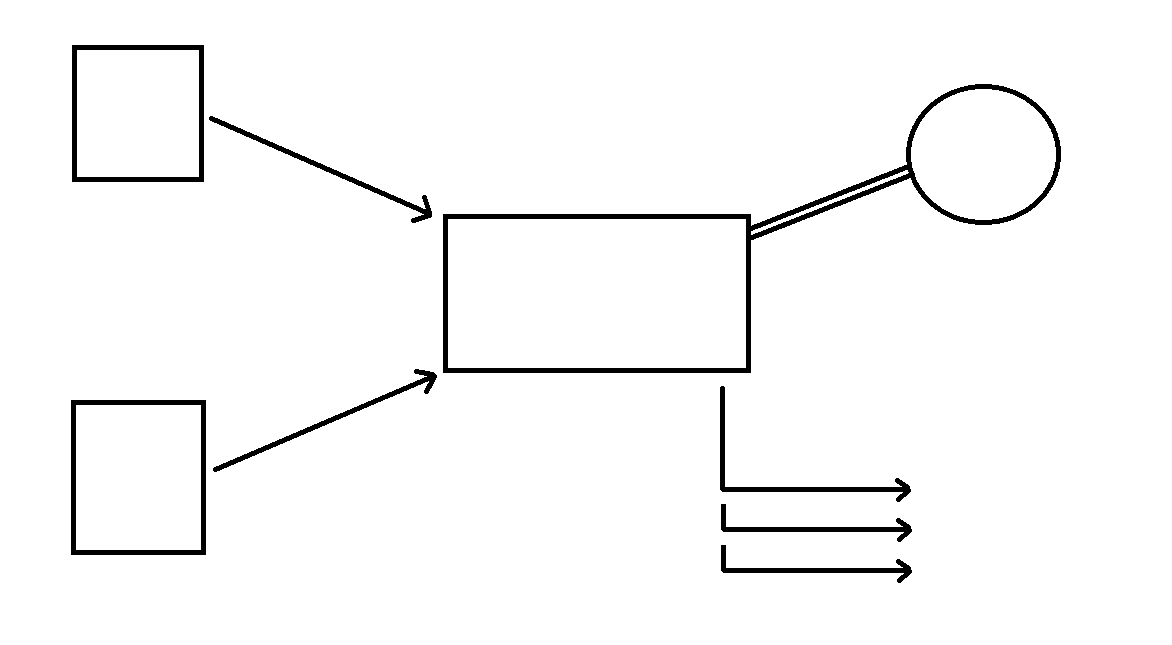
\includegraphics[height=8cm]{presentation/schema}
\end{center}
\caption[schema]{Presentation schema}
\end{figure}

\paragraph*{Paragraphe 1}
~\\
\hskip7mm

Bla

\paragraph*{Paragraphe 2}
~\\
\hskip7mm

Bla

\paragraph*{Paragraphe 3}
~\\
\hskip7mm

Bla

\newpage
\begin{thebibliography}{9}

   \bibitem{Docker}
          Documentation Docker
          \url{https://docs.docker.com/}.
   \bibitem{HyperV Conteneurs}
          Hyper-V Containers
          \url{https://docs.microsoft.com/en-us/virtualization/windowscontainers}.
   \bibitem{Linux containers}
         Linux Containers
         \url{https://linuxcontainers.org/fr/}.
   \bibitem{Virtual Box}
         Virtual Box
         \url{ https://www.virtualbox.org/}.
   \bibitem{Proxmox VE}
         Proxmox VE
         \url{https://www.proxmox.com/en/}.
   \bibitem{VmWare}
         VmWare
         \url{ http://www.vmware.com/fr.html}.
   \bibitem{QEMU}
         QEMU
         \url{http://www.qemu-project.org/   }.
   \bibitem{Hyper-V}
         Hyper-V
         \url{https://www.microsoft.com/fr-fr/cloud-platform/server-virtualization}.      
   \bibitem{KVM}
         KVM
         \url{https://www.linux-kvm.org/}.
   \bibitem{VMMark}
         VM Mark
         \url{https://www.vmmark.com/products/vmark.html}. 
   \bibitem{VM history}
         VM history par IBM
         \url{http://www.vm.ibm.com/history/ }.
 
   \bibitem{Art1}
          An Analysis of Performance Interference Effects in Virtual Environments
          \url{http://ieeexplore.ieee.org/document/4211036/?arnumber=4211036}
      
   \bibitem{Art2}
          The impact of Docker containers on the performance of genomic pipelines
          \url {https://www.ncbi.nlm.nih.gov/pmc/articles/PMC4586803/}              
   \bibitem{Art3}
          W.Huang, J.Liu, B.Abali, Dhabaleswar K. Panda, "A Case for High Performance Computing with Virtual Machines"     
          \bibitem{Art4}
          P.Luszczek, E.Meek, S.Moore,D.Terpstra, Evaluation of the HPC Challenge Benchmarks in Virtualized environments, Springer Berlin Heidelberg, coll. « Lecture Notes in Computer Science », 29 août 2011 
   \bibitem{Documentation de PTS}
        Documentation de Phoronix test suite.
          \url{https://gist.github.com/anshula/728a76297e4a4ee7688d}.
          
   \bibitem{Site de SaltStack}
        Site officiel de SaltStack
          \url{https://saltstack.com/}.

   \bibitem{Documentation de SaltStack}
         Documentation de SaltStack.
          \url{https://docs.saltstack.com/en/latest/}.
          
   \bibitem{Documentation de SaltStack2}
       
          \url{https://docs.saltstack.com/en/latest/topics/installation/debian.html}.

   \bibitem{Documentation de Phoromatic}
       
          \url{https://www.phoronix-test-suite.com/documentation/phoromatic.html}.
\end{thebibliography}


\end{document}